\section{Dashboards}

The dashboard collection is one of the most visible parts of the platform. There are dashboards for
Kubernetes, storage, networking, Kafka, logging, power devices, databases, and service checks
\cite{lsst-it-k8s-cookbook}. Each one encodes a question that someone needed to answer during an
incident or a commissioning shift.

The breadth matters. Observability cannot stop at application pods. The systems that enable
scientific operations all need to be visible in the same place. Dashboards need to let operators
move across those layers without losing their train of thought.

The collection also includes more local, informal dashboards, built because someone needed to
answer a specific question and the general dashboards were not enough. That is a healthy sign. A
living platform has both the polished general views that everyone uses and the rougher tools that
someone built. Over time, the useful ones get promoted into the standard set.

\begin{center}
    \begin{minipage}{0.7\linewidth}
        \centering
        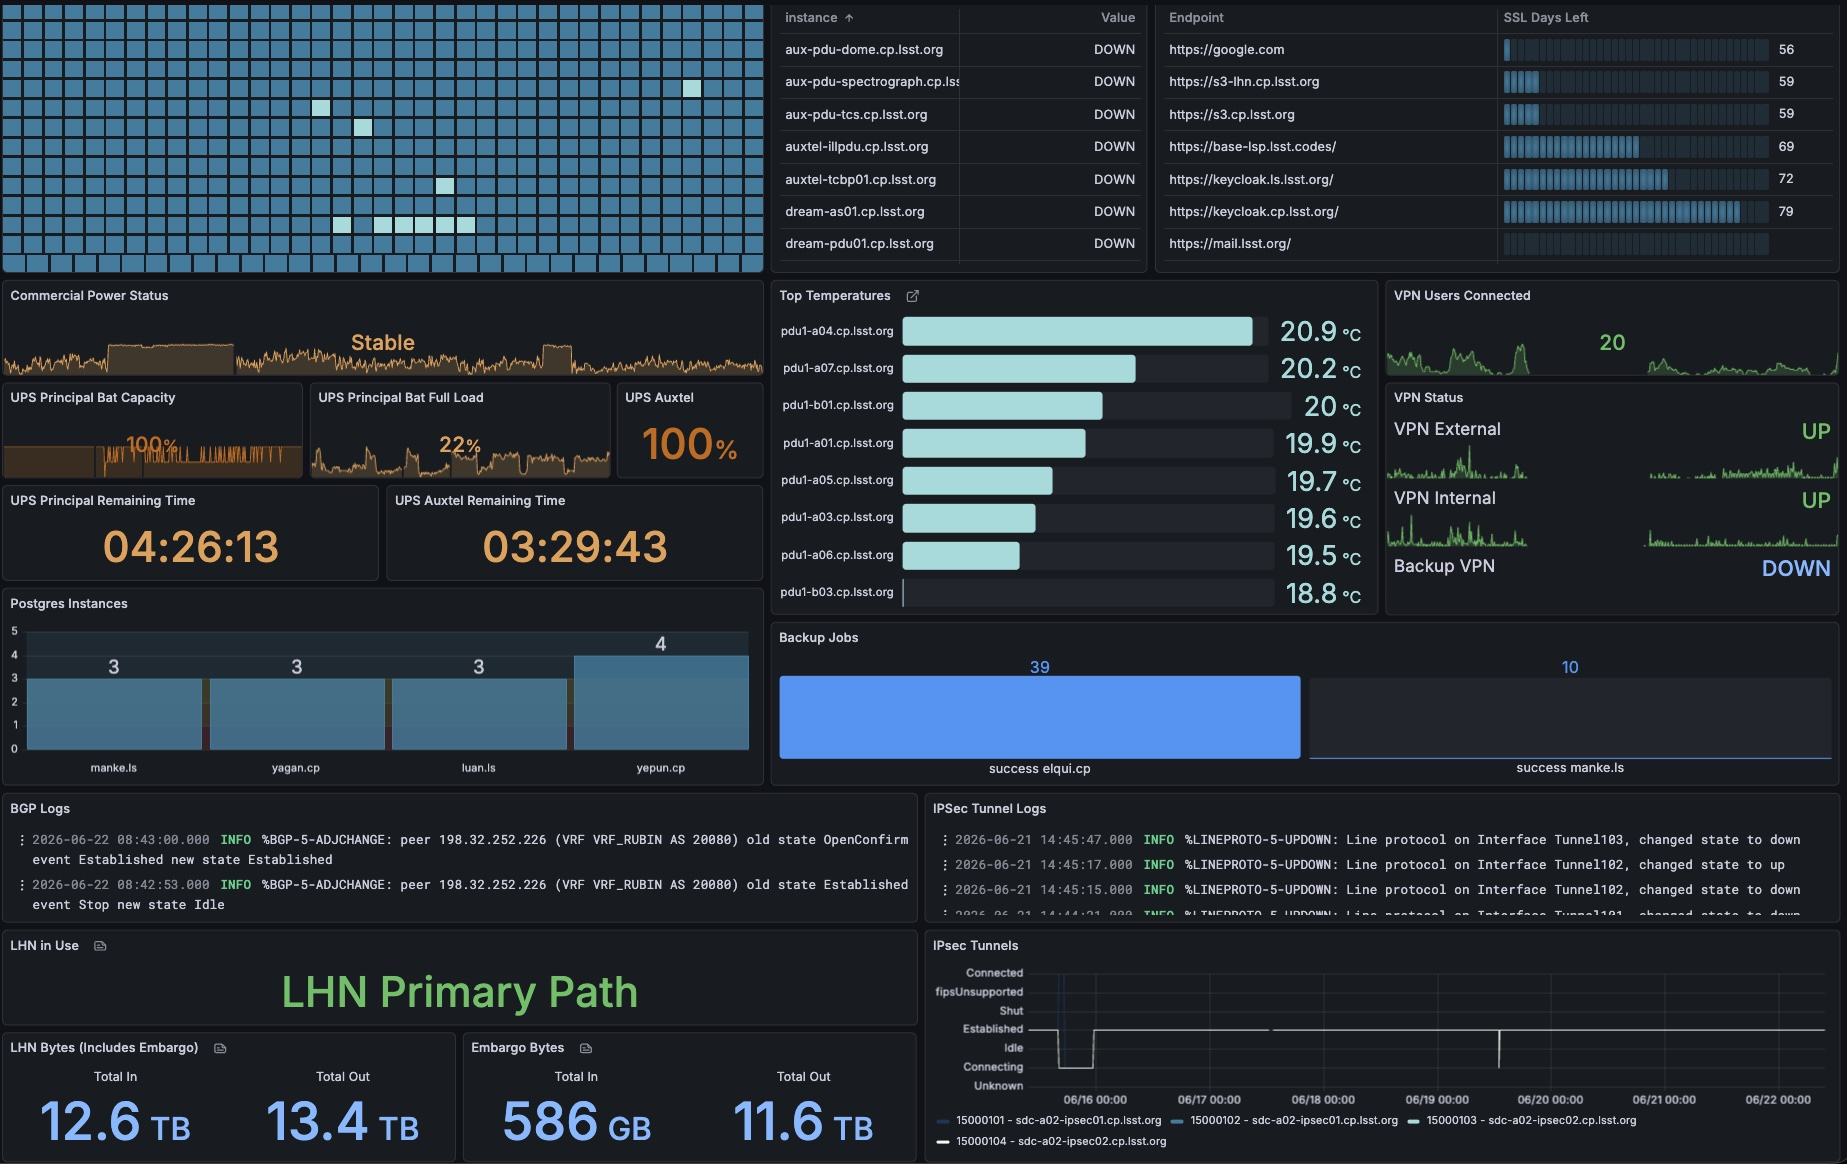
\includegraphics[width=\linewidth]{spie_dashboard.jpg}
        \\[4pt]
        \textbf{Figure 1.} Summary dashboard of several useful metrcis for Engineers and Operators.
    \end{minipage}
\end{center}

One deliberate choice in the dashboard design is color. Every palette used across the dashboards
was selected to be readable under all common forms of color blindness \cite{wcag-color}. This is
not a cosmetic detail; it is an operational requirement. It does not matter how much information a
dashboard contains if the person looking at it cannot immediately tell that something is wrong, or
cannot distinguish between two states at a glance. Any engineer, operator, or scientist at the
observatory should be able to look at a panel and read it correctly, regardless of how they
perceive color.

The difference becomes clear when you simulate how the same dashboard looks under different visual
conditions. Under deuteranopia and protanopia, the two most common forms of red-green color
blindness, the conventional red/green palette collapses \cite{wcag-color}. Red and green become
nearly identical shades of brownish yellow. An operator glancing at the panel during a busy night
has no quick visual cue; they have to stop and read the label to know whether something is up or
down. That extra second matters when you are watching twenty panels at once.

\begin{center}
    \begin{minipage}{0.7\linewidth}
        \centering
        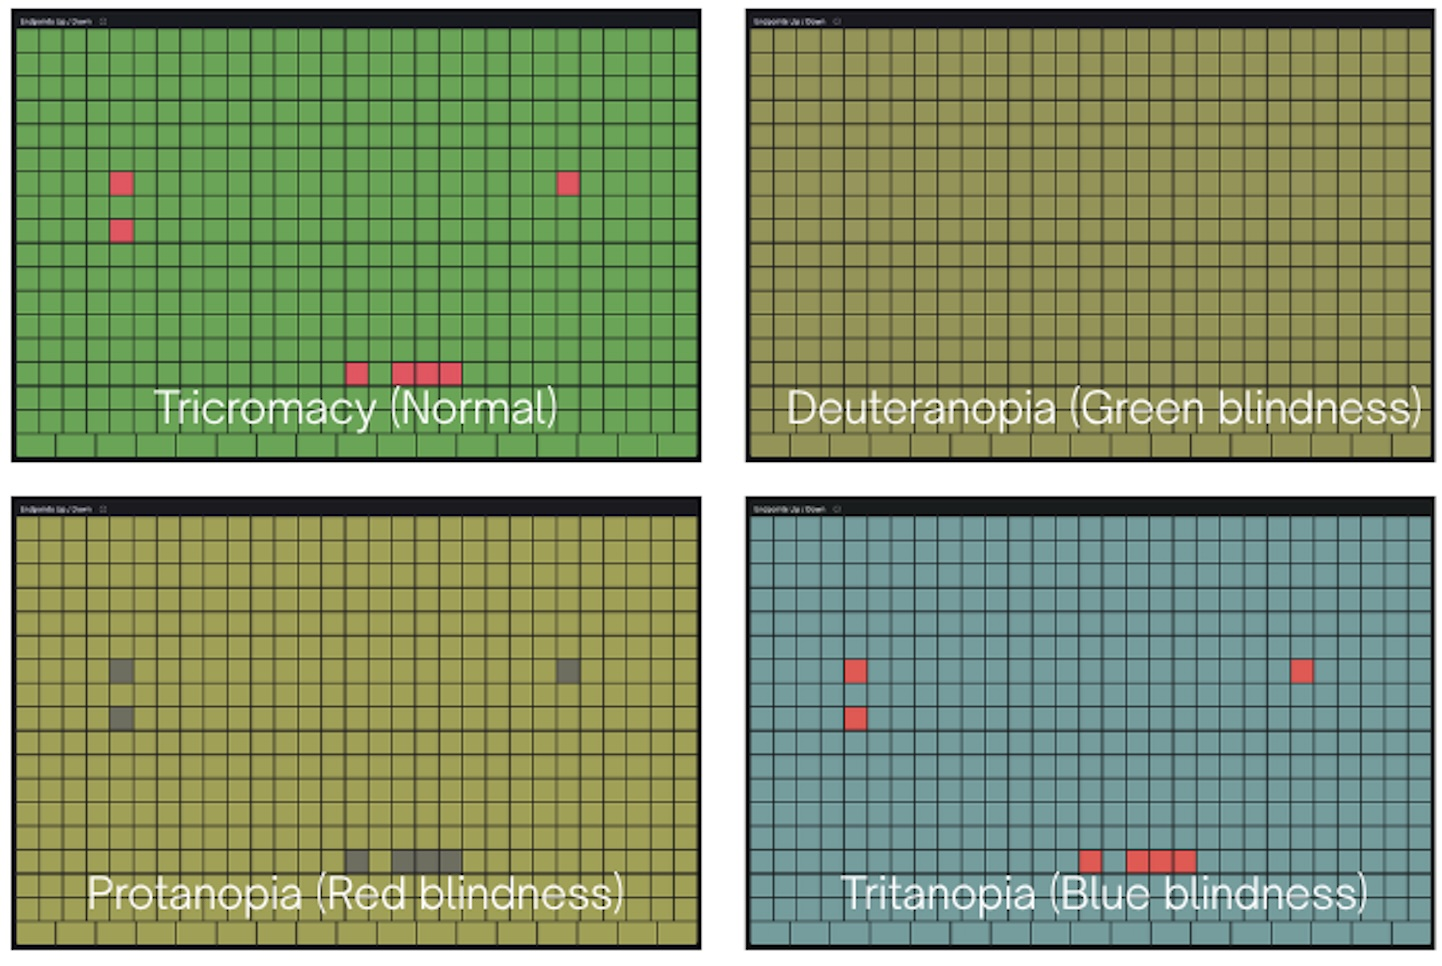
\includegraphics[width=\linewidth]{spie_red.jpg}
        \\[4pt]
        \textbf{Figure 2.} Up and Down monitor using default red and green colors, under different forms of color blindness.
    \end{minipage}
\end{center}

With our palette, the same simulation tells a different story. The colors remain visually distinct
under all tested conditions. The contrast is preserved not only in typical vision but also in
deuteranopia, protanopia, and tritanopia. Someone who has never been able to rely on red and green
to mean anything receives the same immediate signal as everyone else.

\begin{center}
    \begin{minipage}{0.7\linewidth}
        \centering
        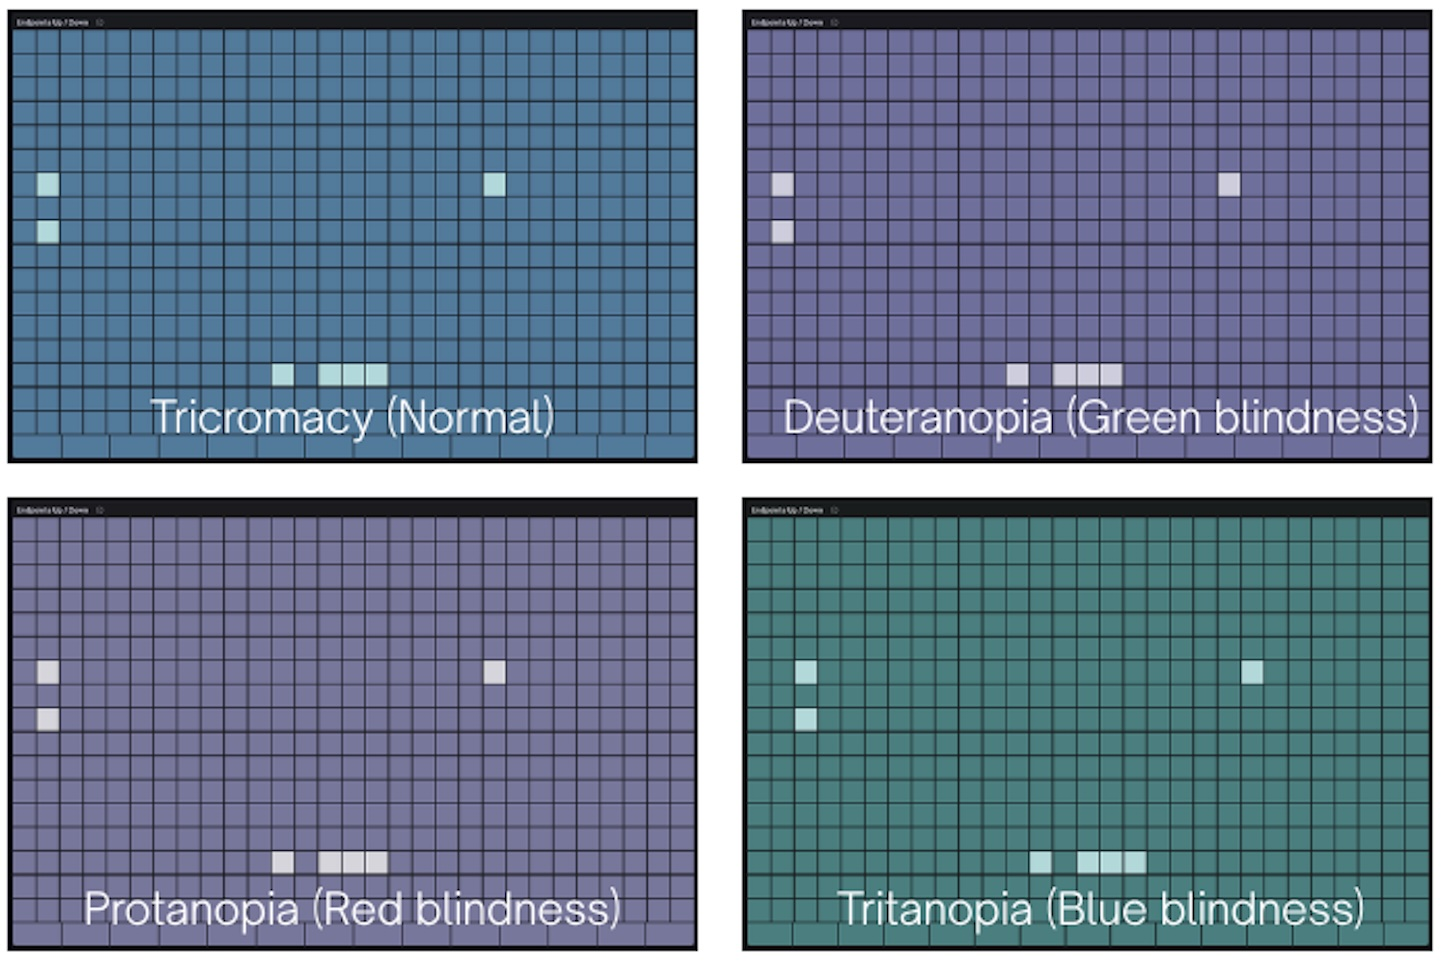
\includegraphics[width=\linewidth]{spie_nored.jpg}
        \\[4pt]
        \textbf{Figure 3.} Up and Down monitor using colors that can be noticeable under different forms of color blindness.
    \end{minipage}
\end{center}

That is the actual goal: not a palette that looks good in a screenshot, but one that works for
every person standing in front of the screens when it matters.

While this development only works with Rubin dashboards, we are exploring how to contribute this
work upstream so it can benefit the broader Grafana community.
